A server hosting a website does not need to operate at its maximum capacity continuously. With proper design and optimization, 
a server can determine when it is necessary to operate at full power and when it can operate in a more energy-efficient manner. 
This approach helps to save energy and reduce operational costs.
However, when transitioning from a lower-power state to full capacity, the server requires a warm-up time to allocate 
resources and reach its optimal performance level. During this warm-up period, the server undergoes initialization processes, 
to prepare itself for handling incoming requests effectively. The warm-up time might impact in a non-negligible way the
performance of the server.\\
\\
\textbf{High Warm-up Time}
A longer warm-up time allows the server to effectively initialize and allocate its resources before the measurement begins. As a 
result, when the measurement period starts, the server is already operating at a high capacity level, enabling it to deliver 
optimal performance.\\
\\
\textbf{Low Warm-up Time}
Conversely to previous situation, a shorter warm-up time can lead the measurement to start before the server reaches
its full potential resulting in lower performance.\\
\\
It is important to note that the impact of warm-up time on server performance can vary due to various factors, such as the specific 
server workload, network conditions, and other environmental variables. As a result, the previously mentioned scenarios regarding the 
relationship between warm-up time and server performance should be interpreted with caution. In this section, we test the warm-up time
impact on different websites performance. For each website different warm-up times were tested with different concurrency levels
(Table \ref{tab:param_warmup}). 

    \begin{table}[H]
        \centering
        \rowcolors{2}{pyblue!25}{white}
            \begin{tabular}{|c|c|}
            \hline
            \rowcolor{pyblue!60}
            \textbf{Parameter} & \textbf{Values} \\
            \hline
            \textbf{Concurrency} & 1, 2, 4, 6, 8, 10 \\
            \textbf{Warm-up (s)} & 2, 4, 6, 8, 10 \\
            \hline
            \end{tabular}
            \caption{\small Parameters warm-up test}
            \label{tab:param_warmup}
    \end{table}

Each experiment was carried out for a duration of 20 seconds, which includes both the actual measurement period and the warm-up time. The used scripts can be consulted 
in the Appendix \ref{sec:scripts}. During 
these experiments, several metrics were recorded to evaluate the performance of the server. The metrics include Requests Per Second (RPS), which measures 
the number of requests processed by the server within a second, Time Per Request (TPR), which calculates the average time taken by the server 
to respond to a single request, and TPR Standard Deviation (SD), which provides an indication of the variability or dispersion of the measured values.
Due to logistic reasons, in this case a 100Mb/s 4G connection from Brescia (BS) was utilized throughout the experiments.\\
In the following sections the results of the experiments are presented and discussed with the help of summarizing charts. To provide an
enhanced perspective of the findings, detailed charts are inserted in the Appendix \ref{sec:detailed_charts}.


\subsubsection{Warm-up time and RPS}
In Figure \ref{fig:5_rps_line}, a consistent pattern is observed across all the websites examined. The Requests Per Second (RPS) metric 
initially increases as the warm-up time is extended, reaching a peak at approximately 6 seconds. However, the delta between the peak and
the neighbors is negligible. Beyond the peak, a slight decrease in RPS can be observed.
The observed behavior can be attributed to several factors. As public websites, the load on these platforms experiences 
significant variations, resulting in fluctuations in the measured results. The complex interaction between user traffic, server capacity,
and network conditions can contribute to the observed patterns in RPS. However, the precise reasons for the slight decrease 
in RPS after the peak are not definitively established and require further investigation.
In conclusion, in the analyzed websites, the RPS metric is not significantly impacted by the warm-up time.\\

    \begin{figure}[H]
        \centering
        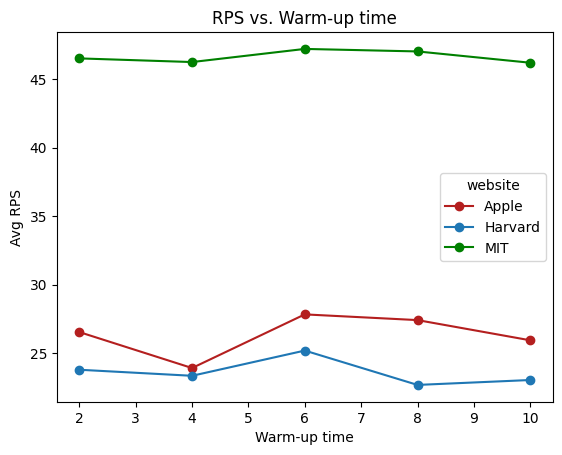
\includegraphics[width=0.48\textwidth]{5_rps_line.png}
        \caption{\small RPS for different warm-up times}
        \label{fig:5_rps_line}
    \end{figure}


\subsubsection{Warm-up time, TPR and SD}
In Figure \ref{fig:5_tpr_line}, the Time Per Request (TPR) metric is shown for different warm-up times. In this case no evident patterns
are observed. It is possible to conclude that in the experiments no correlation appears between the warm-up time and the TPR.\\

    \begin{figure}[H]
        \centering
        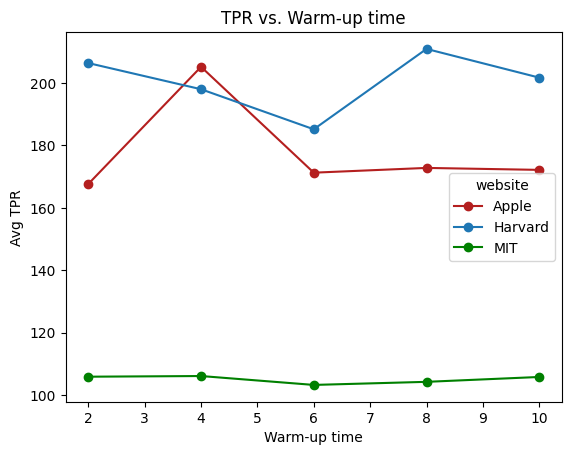
\includegraphics[width=0.48\textwidth]{5_tpr_line.png}
        \caption{\small TPR for different warm-up times}
        \label{fig:5_tpr_line}
    \end{figure}
\noindent
Figure \ref{fig:5_sd_line} presents the TPR Standard Deviation (SD) metric for different warm-up times. Although the pattern may 
not be as pronounced, there appears to be a discernible trend. By dividing the warm-up times into two groups, namely 2 to 5 
seconds and 6 to 10 seconds, it becomes apparent that the SD is higher in the first group. The results indicate that a longer 
warm-up time has a positive impact on the server's performance stability. Indeed, by conceding to the server enough time 
to fully initialize and adapt to the workload, a longer warm-up time facilitates a more stable and predictable performance.

    \begin{figure}[H]
        \centering
        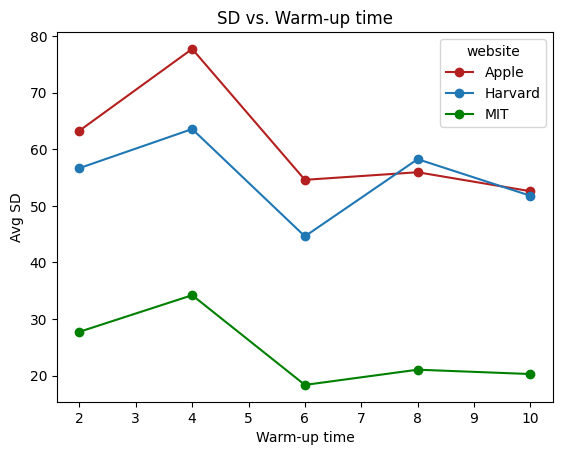
\includegraphics[width=0.48\textwidth]{5_sd_line.png}
        \caption{\small TPR SD for different warm-up times}
        \label{fig:5_sd_line}
    \end{figure}

    In conclusion, while the direct impact of warm-up time on the analyzed websites was not significant within the limitations 
    of the available data, some noteworthy insights into its influence on the RPS and SD metrics were observed. Specifically, 
    a warm-up time of 6 seconds, which accounted for approximately 30\% of the total measurement time, appeared to be associated 
    with a peak in RPS and a decrease in the TPR SD.
    These findings suggest that allocating a sufficient warm-up period for servers can have positive implications for their performance.\\



